% !TeX spellcheck = en_GB
% !TeX program = lualatex
%
% v 2.3  Feb 2019   Volker RW Schaa
%		# changes in the collaboration therefore updated file "jacow-collaboration.tex"
%		# all References with DOIs have their period/full stop before the DOI (after pp. or year)
%		# in the author/affiliation block all ZIP codes in square brackets removed as it was not %         understood as optional parameter and ZIP codes had bin put in brackets
%       # References to the current IPAC are changed to "IPAC'19, Melbourne, Australia"
%       # font for ‘url’ style changed to ‘newtxtt’ as it is easier to distinguish "O" and "0"
%
\documentclass[a4paper,
               %boxit,        % check whether paper is inside correct margins
               %titlepage,    % separate title page
               %refpage       % separate references
               %biblatex,     % biblatex is used
               %keeplastbox,   % flushend option: not to un-indent last line in References
               %nospread,     % flushend option: do not fill with whitespace to balance columns
               %hyphens,      % allow \url to hyphenate at "-" (hyphens)
               %xetex,        % use XeLaTeX to process the file
               %luatex,       % use LuaLaTeX to process the file
               ]{jacow}
%
% ONLY FOR \footnote in table/tabular
%
\usepackage{pdfpages,multirow,ragged2e} %
%
% CHANGE SEQUENCE OF GRAPHICS EXTENSION TO BE EMBEDDED
% ----------------------------------------------------
% test for XeTeX where the sequence is by default eps-> pdf, jpg, png, pdf, ...
%    and the JACoW template provides JACpic2v3.eps and JACpic2v3.jpg which
%    might generates errors, therefore PNG and JPG first
%
\makeatletter%
	\ifboolexpr{bool{xetex}}
	 {\renewcommand{\Gin@extensions}{.pdf,%
	                    .png,.jpg,.bmp,.pict,.tif,.psd,.mac,.sga,.tga,.gif,%
	                    .eps,.ps,%
	                    }}{}
\makeatother

% CHECK FOR XeTeX/LuaTeX BEFORE DEFINING AN INPUT ENCODING
% --------------------------------------------------------
%   utf8  is default for XeTeX/LuaTeX
%   utf8  in LaTeX only realises a small portion of codes
%
\ifboolexpr{bool{xetex} or bool{luatex}} % test for XeTeX/LuaTeX
 {}                                      % input encoding is utf8 by default
 {\usepackage[utf8]{inputenc}}           % switch to utf8

\usepackage[USenglish]{babel}

%
% if BibLaTeX is used
%
\ifboolexpr{bool{jacowbiblatex}}%
 {%
  \addbibresource{jacow-test.bib}
  \addbibresource{biblatex-examples.bib}
 }{}
\listfiles

%%
%%   Lengths for the spaces in the title
%%   \setlength\titleblockstartskip{..}  %before title, default 3pt
%%   \setlength\titleblockmiddleskip{..} %between title + author, default 1em
%%   \setlength\titleblockendskip{..}    %afterauthor, default 1em
\usepackage[acronym]{glossaries}

\newglossaryentry{hc}
{
    name={HC},
    description={harmonic cavity},
    first={\glsentrydesc{hc} (\glsentrytext{hc})},
    plural={HCs},
    descriptionplural={harmonic cavities},
    firstplural={harmonic cavities (\glsentryplural{hc})}
}
\newglossaryentry{hom}
{
    name={HOM},
    description={higher-order mode},
    first={\glsentrydesc{hom} (\glsentrytext{hom})},
    plural={HOMs},
    descriptionplural={higher-order modes},
    firstplural={higher-order modes (\glsentryplural{hom})}
}

\begin{document}

\title{Optimizing Touschek lifetime with overstretched bunch profiles in the MAX IV 1.5 GeV ring}

\author{M. B. Alves\thanks{murilo.alves@lnls.br}\textsuperscript{1}, Brazilian Synchrotron Light Laboratory--LNLS, Campinas, Brazil\\
		F. Cullinan , Å. Andersson, MAX IV Laboratory, Lund, Sweden\\
		\textsuperscript{1}also at Gleb Wataghin Institute of Physics, University of Campinas--UNICAMP, Campinas, Brazil}
\maketitle

%
\begin{abstract}
Synchrotron light sources often use higher-harmonic rf cavities for bunch lengthening to enhance Touschek lifetime. By adjusting the harmonic voltage, a flat-potential condition for the longitudinal voltage can be achieved, typically improving Touschek lifetime by 4 to 5 times. It is known that exceeding the flat-potential voltage results in double-peaked bunch profiles, referred to as overstretched conditions. Simulations suggest overstretched profiles can surpass flat-potential improvements on lifetime. In this paper we report on experimental results from the MAX IV~\SI{1.5}{\giga\electronvolt} storage ring, demonstrating a longer beam lifetime with a stable beam in overstretched conditions compared to the flat-potential case. Additionally, a remarkable agreement between measured bunch profiles using a streak camera and predictions from a semi-analytical equilibrium solver was obtained for all tested harmonic voltages.
\end{abstract}

\section{Ring parameters}
MAX IV is a synchrotron light source facility in Lund, Sweden. The complex has two storage rings, one operating at~\SI{1.5}{\giga\electronvolt} and the other is a fourth-generation ring operating at~\SI{3.0}{\giga\electronvolt}~\cite{MAXIVreport}. This work is focused on lifetime improvement with~\glspl{hc} in the~\SI{1.5}{\giga\electronvolt} ring, whose relevant parameters for these studies are presented in Table~\ref{tab:params}. Two passive normal-conducting \glspl{hc} operating close to the third-harmonic of the rf frequency are installed in the ring.
\begin{table}[!hbt]
   \centering
    \caption{Main parameters for the MAX IV~\SI{1.5}{\giga\electronvolt} ring.}
   \begin{tabular}{lcc}
       \toprule
        Energy  & $E_0$  & $\SI{1.5}{\giga\electronvolt}$  \\
        % Current & $I_0$ & $\SI{300}{\milli\ampere}$ \\
        rf frequency & $f_{\mathrm{rf}}$ & $\SI{99.931}{\mega\hertz}$ \\
        Harmonic number & $h$ & 32 \\
        Momentum compaction & $\alpha$ & $\SI{3.05e-3}{}$ \\
        Energy spread & $\sigma_\delta$ & $\SI{7.45e-4}{}$ \\
        Energy loss per turn& $U_0$ & $\SI{114.4}{\kilo\electronvolt}$ \\
        % \midrule
        % \gls{hc}rf harmonic &  & 3 \\
        % Number of \glspl{hc} &  & 2 \\
        \gls{hc} shunt impedance ($V^2/P$) & $R_s$ & $\SI{5.5}{\mega\ohm}\slash$cavity \\
        \gls{hc} quality factor & $Q$ & $\SI{20800}{}$ \\
        \bottomrule
    \end{tabular}
    \label{tab:params}
\end{table}
\section{Voltage calibration}
\subsection{Main cavities}
With a low-current single-bunch stored in the ring and the \glspl{hc} parked (no \gls{hc} fields), the synchrotron frequency was measured as~$f_s = \SI{7.18}{\kilo\hertz}$. For a single-rf system, the relation between synchrotron frequency and main rf voltage is well-known~\cite{Sands}. Given a measured value of synchrotron frequency $f_s$, the relation can be inverted to determine the main voltage:
\begin{equation}
    V_\mathrm{rf} = \left[\left(\frac{f_s}{f_\mathrm{rf}}\right)^4 \left(\frac{\alpha}{2\pi h E_0}\right)^2 + U_0^2\right]^{1/2}.
\end{equation}
For the parameters of Table~\ref{tab:params}, the measured synchrotron frequency corresponds to a main rf voltage of~$V_\text{rf} = \SI{522.3}{\kilo\volt}$. This value was used throughout the analysis.

\subsection{Harmonic cavities}
For zero detuning and uniform fill, the peak \gls{hc} voltage should be simply~$V_{\mathrm{HC}} = R_s I_0$~\cite{Byrd2001}, where~$R_s$ is the \gls{hc} shunt impedance and~$I_0$ is the stored beam current.
To calibrate the voltage of the \glspl{hc} ,~$\SI{2.3}{\milli\ampere}$ was accumulated uniformly in the ring and the \glspl{hc} were tuned to resonance. This was achieved by maximizing the \gls{hc} voltage readouts. The stored current was then reduced in steps to~$\SI{0.3}{\milli\ampere}$ using a beam scraper and the corresponding \gls{hc} voltages were recorded for each current value. For each current, the \glspl{hc} tuning was adjusted to keep the cavities on resonance.
A linear calibration curve was obtained from the measured \gls{hc} voltage in hardware units vs. expected voltage by $R_s I_0$.
\section{Fitting harmonic voltages from streak-camera measurements}
The bunch profiles were measured with a streak-camera. The streak-camera provides a 2d image with an axis corresponding to a fast scan, with a timescale within bunch separations ($\SI{}{\nano\second}$) and an axis related to a slow scan, with a timescale within a revolution period ($\SI{}{\micro\second}$)~\cite{Brosi:IFAST22}. In Fig.~\ref{fig:streak_camera_image} an example streak-camera image is shown. The time axis can be converted to the~$z$-coordinate by $\tau = z/c$, where $c$ is the speed of light.
\begin{figure}
    \centering
    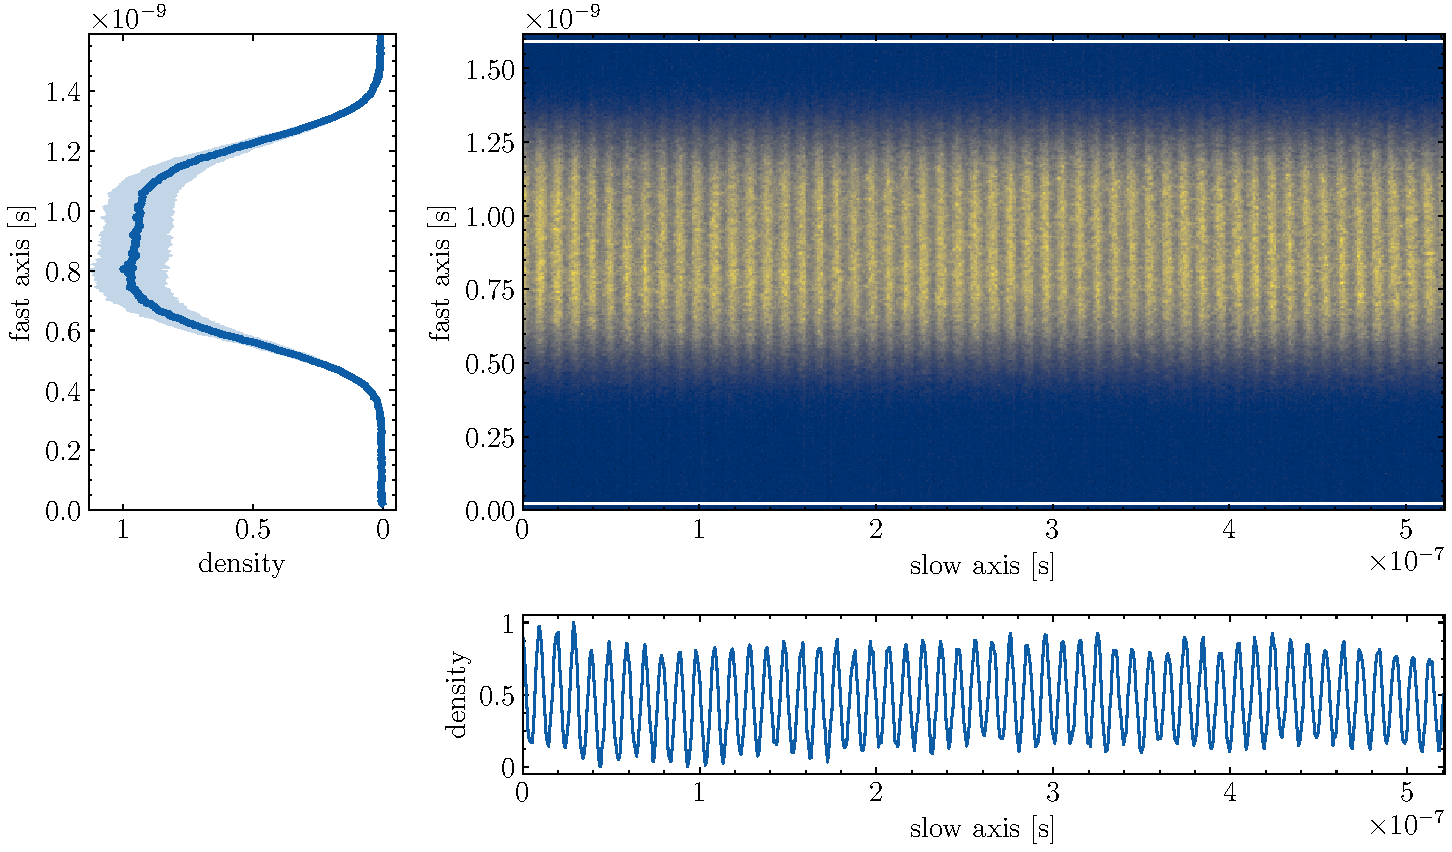
\includegraphics[width=0.45\textwidth]{WEPR42_f1.pdf}
    \caption{Example of streak-camera image acquired with $\SI{200}{\milli\ampere}$ in uniform fill. Left: the solid curve is the average projection along the slow axis and the shaded region is the std variation over bunches.}
    \label{fig:streak_camera_image}
\end{figure}

The equilibrium bunch profiles in the presence of \gls{hc} voltage can be calculated by solving self-consistently the Haissinski equation~\cite{AlvesSa2023}. Let $\lambda_{\text{meas}}(z_i)$ be the measured bunch profile along the axis $z_i$ and averaged over bunches. The goal was to find the \gls{hc} voltage that best reproduces the measured bunch profile. Two fitting parameters were used: the \gls{hc} voltage $V_{\mathrm{fit}}(z)$ (amplitude and phase determined by the \gls{hc} detuning) and an offset $z_{\mathrm{fit}}$ to match the measured and simulated $z_i$-axis. This offset was included as an optional fitting parameter just to automatically account for the undetermined offsets between the axis.

The \gls{hc} voltages were obtained by solving the least-squares minimization problem:
\begin{equation}
\chi^2 = \sum_i \left[\lambda_{\text{meas}}(z_i) - \lambda(z_i - z_{\mathrm{fit}}, V_\mathrm{fit})\right]^2,
\end{equation}
where $\lambda(z, V_\mathrm{fit})$ is the equilibrium bunch distribution calculated in the double-rf system. We noted the same results were obtained when including beam-loading voltage from main cavities and, for simplicity, only beam-loading from \glspl{hc} was considered.

A comparison between measured and calculated bunch profiles is presented in Fig.~\ref{fig:comparison_fit}.
\begin{figure}
    \centering
    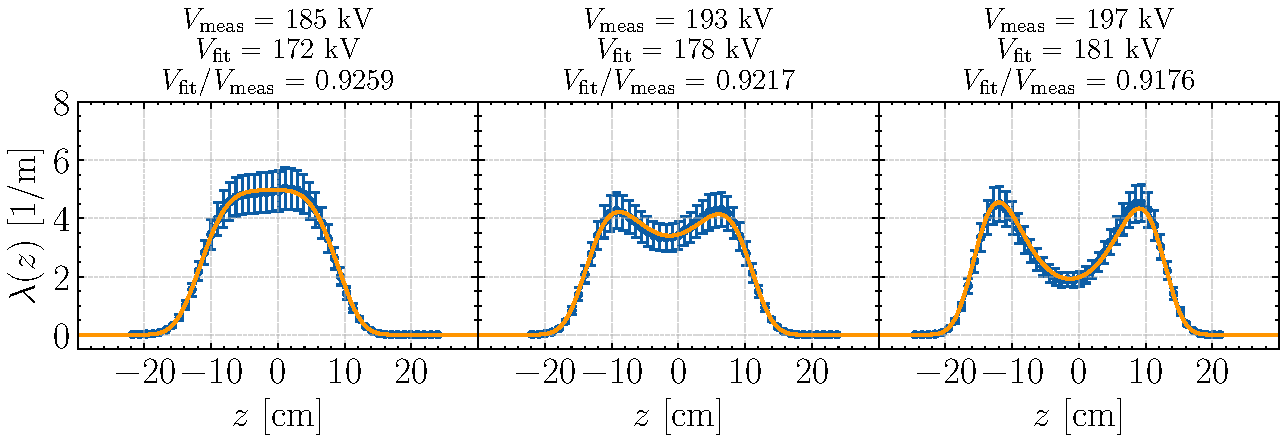
\includegraphics[width=0.4\textwidth]{WEPR42_f2.pdf}
    \caption{Measured and calculated bunch profiles for \SI{200}{\milli\ampere}. Dots represent the average and error bars represent the variation of charge densities over bunches.}
    \label{fig:comparison_fit}
\end{figure} The \gls{hc} voltages needed to match the calculated and measured bunch profiles are systematically lower than the measured voltages. A constant difference could be explained by an error in the shunt impedance considered in the calibration, for example. However, the discrepancy increases linearly with the total voltage\footnote{The calibration of \gls{hc} voltages was measured at low currents, setting the cavities on resonance which is impossible at higher currents. The discrepancy makes us question the validity of this linear calibration curve for higher currents. Perhaps some non-linearity in the voltage measurement device in the cavity could explain a non-linear calibration curve.}, as shown in Fig.~\ref{fig:vfit_vmeas}.\begin{figure}
    \centering
    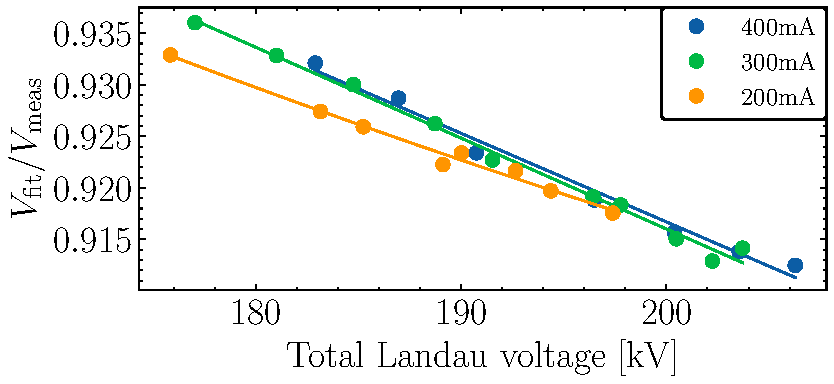
\includegraphics[width=0.4\textwidth]{WEPR42_f3.pdf}
    \caption{Ratio between calculated and measured \gls{hc} voltages for fitting bunch profiles at different beam currents.}
    \label{fig:vfit_vmeas}
\end{figure}

Based on the difference between fit and measured voltages, the linear coefficient of \gls{hc} voltage calibration curve was readjusted by a factor $0.93$. This makes the total measured voltage of~\SI{180}{\kilo\volt} match with the value that reproduces the measured bunch profiles. However, a small discrepancy that increases with the voltage remains, reaching an error of $0.915/0.93 = 0.98$ for the highest measured voltage of~\SI{210}{\kilo\volt}. The adjustment of~$0.93$ could be interpreted as if the actual shunt impedance of the two \glspl{hc} is~\SI{5.115}{\mega\ohm}, i.e., 7\% lower than the value of \SI{5.5}{\mega\ohm} considered previously. This estimated error is considerably larger than bench measurements indicate. Even so, for this study, the \gls{hc} voltage values were adjusted by the~$0.93$ factor.

\section{Lifetime optimization}
The increment in Touschek lifetime due to the bunch lengthening provided by the \glspl{hc} can be estimated by~\cite{Byrd2001}:
\begin{equation}
    \frac{\tau_\text{HC}}{\tau_0} = \frac{\int{\lambda^2_0(z)dz}}{\int{\lambda^2_\text{HC}(z)dz}},
    \label{eq:lifetime}
\end{equation}
where $\lambda_0(z), \lambda_\text{HC}(z)$ are the normalized bunch profiles without and with \gls{hc} fields, respectively. This calculation assumes that the effect of \glspl{hc} on energy acceptance is small, which is typically a good approximation.

It is known from simulations that profiles corresponding to \gls{hc} voltages higher than the flat potential case can be better for lifetime improvement~\cite{AlvesSa2023, Penco2006}. In this condition, referred as overstretched, the bunch profiles have a double-peaked shape. To investigate this experimentally, the \gls{hc} voltage was adjusted above flat potential, while measuring the bunch profiles and the beam lifetime as well. For the main rf voltage of~\SI{522.3}{\kilo\volt} used during the experiment, the flat potential \gls{hc} voltage is~\SI{169.3}{\kilo\volt}. The measurements were carried out with three different values of stored currents in uniform fill.

In the first run with \SI{200}{\milli\ampere}, we observed that for~\SI{185}{\kilo\volt} (9\% above the flat potential voltage), a coupled-bunch mode-0 instability was excited, probably a Robinson instability driven due the small detuning of the harmonic cavities (\SI{130}{\kilo\hertz} in this case). The mode-0 instability limited the maximum value of \gls{hc} voltage for the scan at~\SI{200}{\milli\ampere}. Figure~\ref{fig:200mA_profiles} show the results for the first sequence of measurements.\begin{figure}
    \centering
    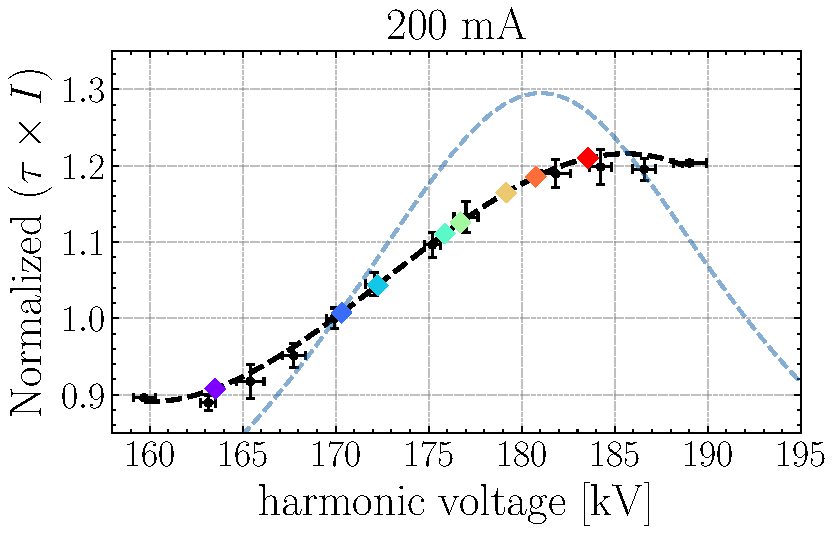
\includegraphics[width=0.4\textwidth]{WEPR42_f4a.pdf}
    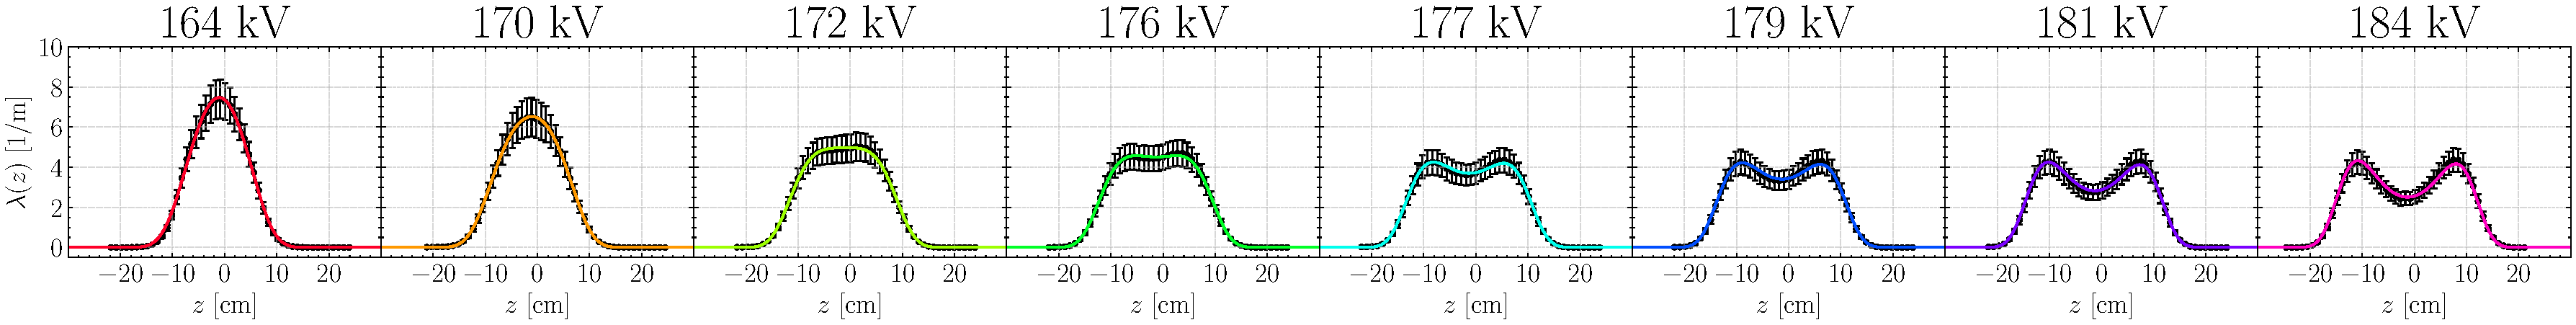
\includegraphics[width=0.48\textwidth]{WEPR42_f4b.pdf}
    \caption{Experimental results of the product lifetime $\times$ current, normalized by the same product measured with \gls{hc} voltage of \SI{170}{\kilo\volt} (flat potential). Measurement carried out with~\SI{200}{\milli\ampere} in the ring. The normalization value is~$(\tau \times I)_\text{flat} = \SI{4604}{\milli\ampere\hour}$, corresponding to a total lifetime of~\SI{23}{\hour} at~\SI{200}{\milli\ampere}. The blue dashed curve is the calculated lifetime from Eq.~\eqref{eq:lifetime} with the corresponding bunch profiles for each \gls{hc} voltage. The black dots and error bars represent the mean and variation of voltage measured in a short period, respectively. The colored markers indicate the voltages in which bunch profile measurements were taken. The sequence of measured and calculated profiles for each \gls{hc} voltage is presented in the bottom plots.}
    \label{fig:200mA_profiles}
\end{figure}

For the second run, the stored current was increased to~\SI{300}{\milli\ampere}. At higher currents the same \gls{hc} voltage is achieved with a larger detuning, thus the Robinson instability could be avoided. However, for~\SI{188}{\kilo\volt}, coupled-bunch instabilities were excited by \glspl{hom} of the \glspl{hc}. After temperature tuning of \glspl{hc} , the \glspl{hom}' frequencies shifted and the instabilities were suppressed. At the new operating temperatures, it was possible to further increase the \gls{hc} voltage while keeping the beam stable. The results obtained at~\SI{300}{\milli\ampere} are shown in Fig.~\ref{fig:300mA_profiles}, where the negative impact of the coupled-bunch instabilities on lifetime is evident at~\SI{188}{\kilo\volt}.
\begin{figure}
    \centering
    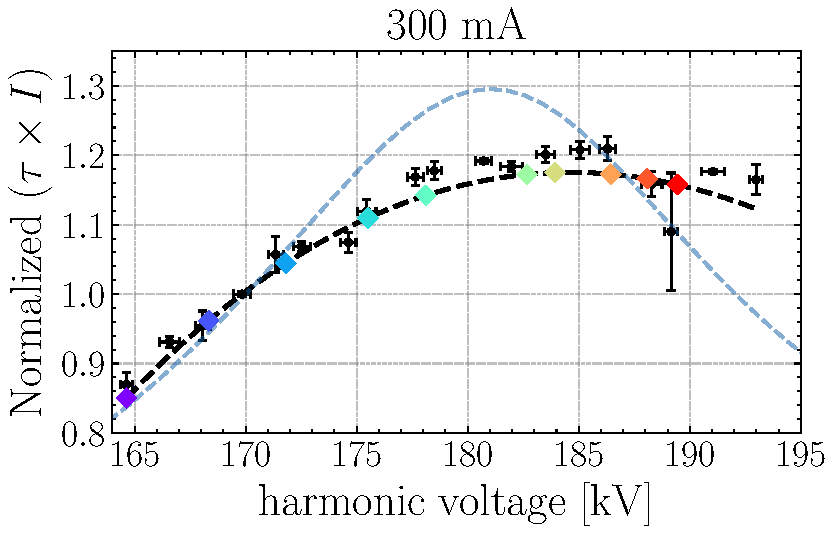
\includegraphics[width=0.4\textwidth]{WEPR42_f5a.pdf}
    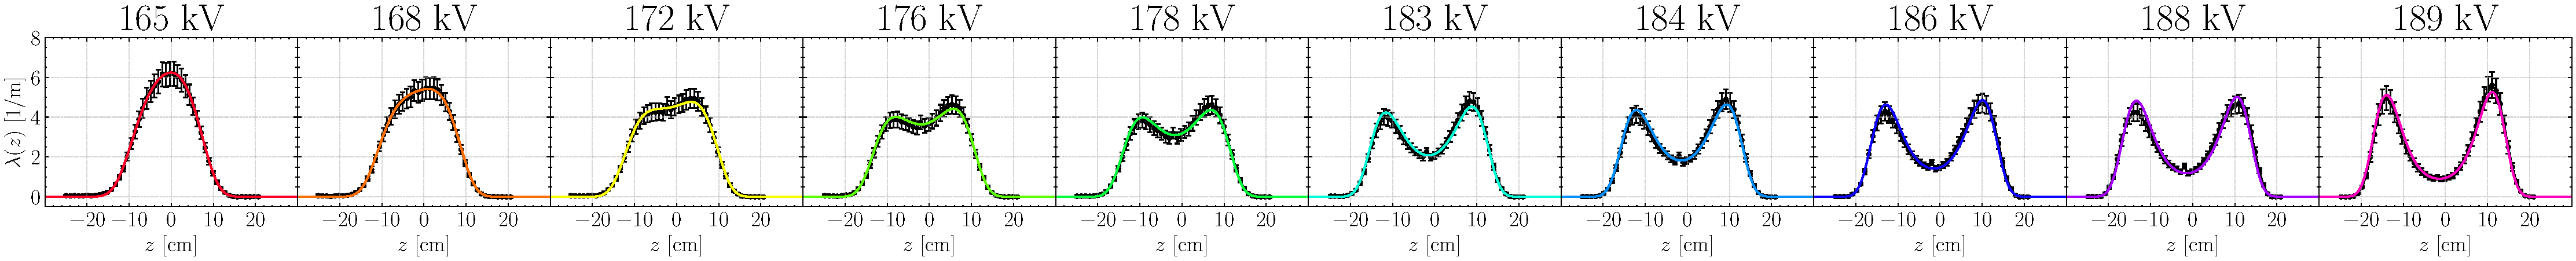
\includegraphics[width=0.48\textwidth]{WEPR42_f5b.pdf}
    \caption{Same experiment as shown in Fig.~\ref{fig:200mA_profiles} with a higher current of~\SI{300}{\milli\ampere}. The normalization value measured with \gls{hc} voltage of \SI{170}{\kilo\volt} is~$(\tau \times I)_\text{flat} = \SI{5712}{\milli\ampere\hour}$, corresponding to a lifetime of~\SI{19}{\hour} at~\SI{300}{\milli\ampere}.}
    \label{fig:300mA_profiles}
\end{figure}

% 200mA --> 4604 mAh, max 6250 mAh
% 300mA --> 5712 mAh, max 6907 mAh
% 400mA --> 4642 mAh, max 5945 mAh

A final set of measurements at~\SI{400}{\milli\ampere} was made. The temperature tuning that cured the coupled-bunch instabilities at~\SI{300}{\milli\ampere} was maintained. Different from the other two cases, the initial value of \gls{hc} voltage was already set to flat potential voltage of~\SI{170}{\kilo\volt}, taking into account the identified calibration error. No instabilities were experienced in this run and the results are shown in Fig.~\ref{fig:400mA_profiles}.
\begin{figure}
    \centering
    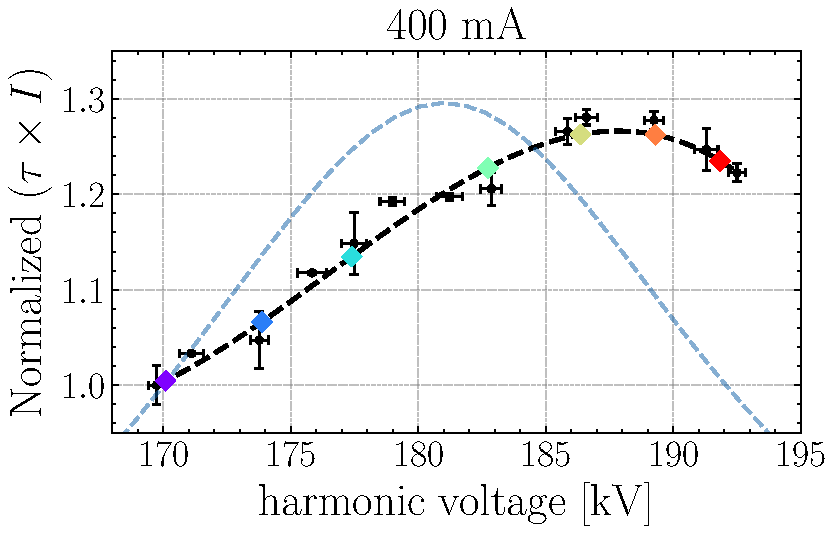
\includegraphics[width=0.4\textwidth]{WEPR42_f6a.pdf}
    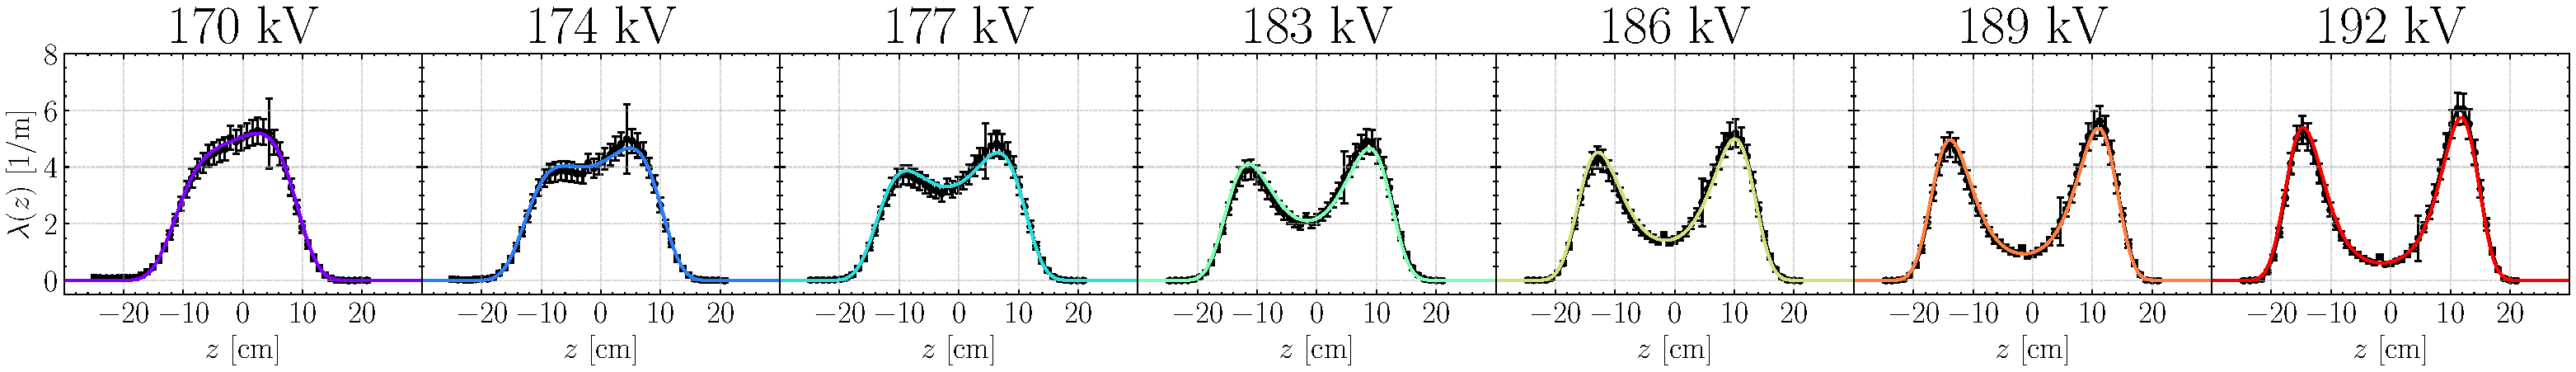
\includegraphics[width=0.48\textwidth]{WEPR42_f6b.pdf}
    \caption{Same experiment as shown in Figs.~\ref{fig:200mA_profiles} and~\ref{fig:300mA_profiles} with a higher current of~\SI{400}{\milli\ampere}. The normalization measured with~\SI{170}{\kilo\volt} of \gls{hc} voltage is~$(\tau \times I)_\text{flat} = \SI{4642}{\milli\ampere\hour}$, corresponding to a lifetime of~\SI{11.6}{\hour} at~\SI{400}{\milli\ampere}. The point close to~$z=\SI{5}{\centi\meter}$ with large variation in intensity should be just an artifact from the streak-camera acquisition.}
    \label{fig:400mA_profiles}
\end{figure}
\section{Discussion and conclusion}
The results shown in Figs.~\ref{fig:200mA_profiles},~\ref{fig:300mA_profiles} and~\ref{fig:400mA_profiles} confirm that operating with \gls{hc} voltages beyond the flat potential can help to improve beam lifetime. Moreover, we were able to find in simulation the \gls{hc} voltages that produced bunch profiles in close agreement with streak-camera measurements. This fitting process has the potential to be useful as a beam-based calibration of \gls{hc} voltages at high current. Benchmarking against other calibration methods is required for validation.

Experiments with stored beam currents of \SI{200}{\milli\ampere} and \SI{300}{\milli\ampere} were limited by beam instabilities. The product (lifetime~$\times$ current) was higher with \SI{300}{\milli\ampere} compared to \SI{200}{\milli\ampere} and \SI{400}{\milli\ampere}, suggesting that other uncontrolled factors were affecting the lifetime in this case. Interestingly, the beam remained stable at the highest current of \SI{400}{\milli\ampere}, allowing acquisitions with highly overstretched bunches.

Overall, the observed improvement in lifetime with \glspl{hc} did not match the theoretical expectation based on Eq.~\eqref{eq:lifetime}. The best \gls{hc} voltage for lifetime was consistently higher than expected and the range of voltages producing longer lifetimes in practice is broader than predicted. This could be because Eq.~\eqref{eq:lifetime} assumes that, except for the longitudinal density, all parameters remain constant, while they may vary in reality. Additionally, the formula only considers the impact of \glspl{hc} on Touschek lifetime, while the total lifetime was measured. Further studies are needed to investigate these differences.

\section{Acknowledgments}
The authors thank Miriam Brosi for the support with the streak-camera setup and for providing the code for data processing. M.~B.~Alves acknowledges FINEP for the research conducted at MAX IV, under the Grant FINEP/MAXSIRIUS nº~01.18.0007.00.
\ifboolexpr{bool{jacowbiblatex}}%
	{\printbibliography}%
	{%
	% "biblatex" is not used, go the "manual" way

	%\begin{thebibliography}{99}   % Use for  10-99  references
	\begin{thebibliography}{9} % Use for 1-9 references

    \bibitem{MAXIVreport}
    MAX IV Detailed Design Report,
    \url{https://www.maxiv.lu.se/beamlines-accelerators/accelerators/accelerator-documentation-2/}

    \bibitem{Sands}
    M. Sands,
    ``The Physics of Electron Storage Rings: An Introduction''
    \emph{Conf. Proc. C} \textbf{6906161}, 257--411 (1969),
    SLAC-R-121, SLAC-121.

    \bibitem{Brosi:IFAST22}
    M. Brosi,
    ``Diagnosing collective effects in the MAX IV storage rings''
    presented at I.FAST, Karlsruhe, 2022,
    \url{https://indico.scc.kit.edu/event/2592/contributions/10368/attachments/5037/7789/IFAST_presentation_mbrosi.pdf}

    \bibitem{AlvesSa2023}
    M. B. Alves and F. H. de S\'a,
    ``Equilibrium of longitudinal bunch distributions in electron storage rings with arbitrary impedance sources and generic filling patterns''
    \emph{Phys. Rev. Accel. Beams 26}, 094402 (2023)

    \bibitem{Byrd2001}
    J. M. Byrd and M. Georgsson,
    ``Lifetime increase using passive harmonic cavities in synchrotron light sources''
    \emph{Phys. Rev. ST Accel. Beams} \textbf{4}, 030701 (2001),
    \url{https://link.aps.org/doi/10.1103/PhysRevSTAB.4.030701}.

    \bibitem{Penco2006}
    G. Penco and M. Svandrlik,
    ``Experimental studies on transient beam loading effects in the presence of a superconducting third harmonic cavity''
    \emph{Phys. Rev. ST Accel. Beams} \textbf{9}, 044401 (2006),
    \url{https://link.aps.org/doi/10.1103/PhysRevSTAB.9.044401}.

	\end{thebibliography}
} % end \ifboolexpr

\end{document}
